\documentclass{llncs}

%\usepackage{polyglossia} % Must come before biblatex
\usepackage{algorithm}
\usepackage{algpseudocode}
\usepackage{amsfonts}
\usepackage{amsmath}
\usepackage{bm}
\usepackage{booktabs}
\usepackage{csquotes}
\usepackage[T1]{fontenc}
%\usepackage{fontspec}
\usepackage{graphicx}
\usepackage{hyperref}
%\usepackage{lua-visual-debug}
\usepackage{tabularx}


%\setdefaultlanguage{english}
%\setotherlanguage{czech}

\hypersetup{
	pdfencoding=auto,
	unicode=true,
	bookmarksopen=true,
	bookmarksopenlevel=3
}

\newcommand{\name}[1]{\textit{#1}}
\newcommand{\mathfield}{\ensuremath{\mathbb}}
\newcommand{\mathmat}{\ensuremath{\mathbf}}
\newcommand{\mathset}{\ensuremath{\mathbb}}
\newcommand{\mathspace}{\ensuremath{\mathcal}}
\newcommand{\mathvec}{\ensuremath{\bm}}

\newcounter{enumroman}
\newenvironment{romanitems}{\begin{list}{\bfseries(\roman{enumroman})\hfill}{\usecounter{enumroman}\setlength{\labelwidth}{\leftmargin}\addtolength{\labelwidth}{-1\labelsep}\topsep=0mm plus 2pt\itemsep=0mm\parsep=0mm plus 2pt\itemindent=0mm}}{\end{list}}

\DeclareMathOperator*{\argmin}{arg\,min}
\DeclareMathOperator*{\argmax}{arg\,max}


\begin{document}

\title{Balancing performance and complexity with adaptive graph coarsening}
\titlerunning{Adaptive graph coarsening}


%\author{
	%Marek Dědič\inst{1 2}\orcidID{0000-0003-1021-8428} \and
	%Lukáš Bajer\inst{2}\orcidID{0000-0002-9402-6417} \and
	%Pavel Procházka\inst{2} \and
	%Martin Holeňa\inst{3}\orcidID{0000-0002-2536-9328}
%}
%\authorrunning{M. Dědič et al.}
\author{}

%\institute{
	%Faculty of Nuclear Sciences and Physical Engineering, Czech Technical University in Prague, Břehová 7, Prague, 110 00, Czech Republic \and
	%Cisco Systems, Inc., Karlovo náměstí 10, Prague, 120 00, Czech Republic \email{\{madedic,lubajer,paprocha\}@cisco.com} \and
	%Institute of Computer Science, Czech Academy of Sciences, Pod vodárenskou věží 2, Prague, 182 07, Czech Republic \email{martin@cs.cas.cz}
%}
\institute{}

\maketitle

\abstract{
Graph based models are used for tasks with increasing size and computational demands. We present a method for studying graph properties from the point of view of a downstream task. This method allows a user to precisely select the resolution at which the graph in question should be coarsened. Our method builds on an existing algorithm for pretraining on coarser graphs, HARP. We extend both main parts of the algorithm in order to observe the effect of graph coarsening to model quality on a fine level. We present a general framework for graph coarsenings, allowing is to cover, apart from HARP, two alternative algorithms based on graph diffusion convolution. Additionally, we present a novel way for refining the reduced graph in a targeted way based on the downstream classification confidence for particular nodes. Together, these enhancements provide sufficient detail where needed, while collapsing structures where per-node information is not necessary for high model performance.
Hence, the method provides a general meta-model for enhancing graph embedding models such as node2vec. We apply it to several datasets, compare the considered coarsenings on them and discuss the differing behaviour on each of them in the context of their properties.
}

\keywords{
  Graph representation learning,
  Graph coarsening,
  Graph diffusion,
  Graph homophily,
  Performance-complexity trade-off,
  HARP
}


\section{Introduction}
Across a wide variety of applications and domains, graphs emerge as a domain-independent and ubiquitous way of organizing structured data. Consequently, machine learning on graphs has, in recent years, seen an explosion in popularity, breadth and depth of both research and applications. While there have been significant advances in algorithms for learning from graph data \cite{defferrard_convolutional_2016,kipf_semi-supervised_2017}, the underlying graph topology has, until recent works \cite{topping_understanding_2021,velickovic_geometric_2021}, received much less attention. In the reported research, we investigate graph granularity in the context of quality of graph embeddings, subsequently reflected in the quality of the downstream node classification relying on those embeddings. The importance of such an investigation follows from the importance of the quality aspect for the downstream task.

Typically, an application of machine learning to graphs has two phases: representation learning, which maps the graph into a Euclidean space, and a downstream task, such as regression, clustering, or, in our case, node classification. The first phase has very high computational demands, which can be substantially decreased with graph coarsening, i.e., merging vertices as a means of decreasing the graph size. However, it is known that there is an interplay between coarsening and the quality of embedding \cite{akyildiz_understanding_2020,makarov_survey_2021}, which in turn entails an interplay between coarsening and the performance of the downstream task.

Our work builds on the HARP method for pretraining on coarsened graphs \cite{chen_harp_2018}. In HARP, a graph is repeatedly coarsened and the coarser graphs are then used in reverse order (from coarsest to finest) to pre-train a graph representation learning algorithm. While HARP itself works with and modifies the graph structure, this is not the main interest of its authors and it does not include any adaptation to the quality of the obtained result as the authors focus more on the representation and classification accuracy for the original graph. In our work, we modify and generalize the HARP framework to closely study the relationship between graph coarsenings and graph quality in terms of the performance of a downstream task -- node classification.

The main contributions of this paper are extensions of the HARP algorithm in both of its two main parts. We present two alternative graph coarsening schemes based on graph diffusion convolution and a novel approach to refining the reduced graph in a targeted way, based on the confidence of downstream classification. This method maximizes performance under limited graph size.

In the next section, related work is discussed, with the exception of HARP, which is the basis of the reported research, therefore it is addressed in detail in Section~\ref{sec:harp-framework}, together with an outline of how it could be extended into a general framework for graph coarsening. Section~\ref{sec:performance-complexity} introduces the addressed performance-complexity trade-off problem. Section~\ref{sec:our-method} is the core of this work, presenting our extension of the prolongation step, as well as several proposed alternative graph coarsening schemes. Finally, all proposals are experimentally verified and compared in Section~\ref{sec:experimental-evaluation}.

\section{Related work}

The publications most relevant to our research are \cite{chen_harp_2018}, in which the HARP approach is proposed, and \cite{gasteiger_diffusion_2019}, in which graph coarsening is performed by means of graph diffusion. Because we directly extend, modify or combine those methods, they will be recalled in some detail in Sections \ref{sec:harp} and \ref{sec:gdc-coarsening}. Other important works concerning graph coarsening are \cite{akyildiz_understanding_2020,chen_graph_2022,cai_graph_2022}, which survey numerous coarsening methods, \cite{huang_scaling_2021}, which presents results concerning scalability of graph coarsening, \cite{catalyurek_multithreaded_2012,herrmann_multilevel_2019}, which establish coarsening as a basis for partitioning, and \cite{loukas_graph_2019}, which shows relationships of graph coarsening to properties of the Laplacian. In view of the fact that the HARP approach, which we extend and modify, is a multilevel approach, we paid attention also to the multilevel graph coarsening methods proposed in \cite{bethune_hierarchical_2020,xie_graph_2020,zhang_harp_2021,liu_hierarchical_2021}, among them \cite{zhang_harp_2021} also being inspired by HARP.

In a broader context, our research is related to the more general topic of graph reduction, which apart from graph coarsening includes also graph sparsification. A general framework covering both coarsening and sparsification has been proposed in \cite{bravo_hermsdorff_unifying_2019}. Also of note is the recent work \cite{kammer_space-efficient_2022}, presenting an alternative coarsening approach for planar graphs and \cite{liu_comprehensive_2022}, which sparsifies not only the graph topology, but simultaneously also the features of its nodes and weights of graph neural network used for its embedding. Elaboration of graph coarsening methods in machine learning can build on several decades of their succesful application, such as pairwise aggregation, independent sets, or algebraic distance, in numerical linear algebra \cite{chen_graph_2022}, including in particular multilevel graph coarsening \cite{osei-kuffuor_matrix_2015,ubaru_sampling_2019}.

\section{The performance-complexity trade-off problem}\label{sec:performance-complexity}

The main aim of this work is to explore the performance-complexity characteristics in the context of graph learning, as considered, for example, in \cite{prochazka_downstream_2022}. Consider an undirected graph \( G \) with nodes \( V \left( G \right) \) and edges \( E \left( G \right) \). The result of the graph coarsening part of the algorithm is a sequence of graphs \( G_0, G_1, G_2, \dots, G_L \) where \( G_0 = G \) and \( L \in \mathfield{N} \) is a hyper-parameter of the method.
Given a model \( M \) that operates on graphs, a performance metric \( P \left( G, M \right) \) and a complexity metric \( C \left( G, M \right) \), the sequence \( G_0, G_1, \dots, G_L \) can be plotted in the performance-complexity space, where the original graph \( G_0 \) usually provides the best performance and incurs the most complexity and subsequent coarsened graphs improve complexity and hurt performance. -- see Figure~\ref{fig:performance-complexity} for an illustration.

\begin{figure}
  \centering
  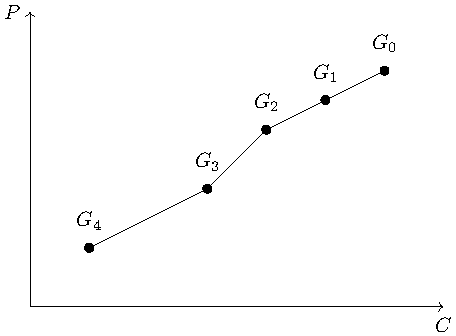
\includegraphics[width=0.45\textwidth]{images/performance-complexity/performance-complexity.pdf}
  \caption{An example of a performance-complexity curve for a sequence of graphs.}
  \label{fig:performance-complexity}
\end{figure}

This performance-complexity characteristic allows for a choice of an optimal \textbf{working point} for the model M -- i.e., the choice of the optimal coarsening level \( G_i \), which directly influences both the performance and the complexity of the model. The choice of the working point is subjective and depends on the particular use-case, downstream task and the environment in which the model is to be deployed. In general, however, two distinct ways of using the characteristic emerge:
\begin{itemize}
  \item Finding the most performant model for a given complexity budget. That is, for a given maximum allowable complexity \( C_\mathrm{max} \), a graph \( G_i \) is to be found that maximizes \( P \left( G_i, M \right) \) while maintaining \( C \left( G_i, M \right) \leq C_\mathrm{max} \).
  \item Finding the least complex model satisfying a performance target. That is, for a given minimum acceptable performance \( P_\mathrm{min} \), a graph \( G_i \) is to be found that minimizes \( C \left( G_i, M \right) \) while maintaining \( P \left( G_i, M \right) \geq P_\mathrm{min} \).
\end{itemize}

\subsection{Choice of the performance and complexity metrics}

The choice of a suitable performace metric \( P \left( G, M \right) \) is dependent on the downstream task in question -- usually, the same metric used to evaluate the downstream model is utilized as the performance metric. In this work, the accuracy of the transductive classification of nodes is chosen as the performance metric.

In practice, two of the most important complexity metrics are computational complexity and memory complexity. These may not only affect the monetary cost and time needed to train a model, but may prevent the application of a considered model outright due to the infeasibility of the given configuration. As shown in \cite{chiang_cluster-gcn_2019}, in the context of graph algorithms, a good proxy for real-world complexity metrics may be the number of edges or the number of nodes in the graph, the latter being the metric used in the rest of this work.

\subsection{Computational complexity of finding the optimal working point}

While the methods proposed in the rest of this work may yield models and graphs with lower computational demands than models using the original graph, the algorithm for finding the optimal working point itself entails running the same complex models on multiple graphs, therefore potentially offsetting any gains from the lower complexity of the model itself. To overcome these potential shortcomings, the following options are considered:
\begin{itemize}
  \item The optimal working point may generalize to datasets other than the one used for the performance-complexity analysis. While this may not in general be said for any two datasets, similar datasets may arise in the practical setting, such as in the domain of computer network security, where a new graph is produced each time the network is scanned and it is reasonable to assume that the working point would be the same for graphs generated in this manner. Generally, this applies especially well in the case of transductive classification where the model needs to be re-trained when the underlying graph changes.
  \item The whole performance-complexity curve is not needed to choose the optimal working point. In the context of this work, the graphs are evaluated in reverse order, i.e. starting with \( G_L \). For the case of a performance target, the evaluation can be stopped after reaching this target. For the other case of a complexity budget, the evaluation is run until the complexity maximum is met, at which point the working point can be selected to maximize performance. In either case, only graphs \( G_b, \dots, G_L \) are evaluated, for some value of \( b \), therefore removing the need to evaluate the model on the graphs with the highest complexity demands.
\end{itemize}

\section{A coarsening framework based on HARP}\label{sec:harp}

HARP is a method for improving the performance of graph representation learning algorithms such as DeepWalk \cite{perozzi_deepwalk_2014}, node2vec \cite{grover_node2vec_2016}, or, in general, any algorithm that produces embeddings as a distinct output. The method is a combination of dataset augmentation and pre-training based on the general principle that graph-based models train more efficiently on smaller graphs and can thus be pre-trained on a coarsened representation of the graph at hand. Moreover, the coarsened graphs are able to approximate the global properties of the original data, enabling the representations to better encapsulate such a global structure.

The sequence \( G_0, G_1, G_2, \dots, G_L \) introduced in Section~\ref{sec:performance-complexity} is generated one step at a time, that is, graph \( G_i \) is generated from the graph \( G_{i - 1} \) by coarsening it -- lowering the number of nodes and edges while preserving in some sense the general structure of the graph. Following \cite{chen_harp_2018}, let \( \varphi_i \) denote the mapping \( G_i = \varphi_i \left( G_{i - 1} \right) \). In this work, we restrict the definition of such a coarsening \( \varphi_i \) to only consist of a series of edge contractions. Therefore, each coarsening corresponds to a set \( \mathcal{C} \subseteq E \left( G \right) \), i.e. a subset of edges of the original graph. This description of a graph coarsening is inspired by \cite{schulz_mining_2019}, which is why it differs from the weaker definition of a graph reduction as selecting a subset of nodes and edges \cite{huang_scaling_2021,loukas_graph_2019}.

In an overview, the HARP algorithm consists of the following steps:

\begin{enumerate}
  \item \textbf{Dataset augmentation}. The graph \( G \) is consecutively reduced in size by the application of several graph coarsening schemas. In each step, the coarsened graph can be viewed as an ever coarser representation of the graph data and its global structure. This step can be run ahead-of-time to produce the resulting coarsened graphs \( G_0, G_1, \dots, G_L \).
\end{enumerate}
After all the coarsened graphs are pre-computed, the method itself can be executed by repeating the following steps on the graphs from the coarsest to the finest (i.e. from \( G_L \) to \( G_0 \)):
\begin{enumerate}\setcounter{enumi}{1}
  \item \textbf{Training on an intermediary graph}. The graph embedding model is trained on \( G_i \), producing \( \Phi_{G_i} \), an embedding of the graph in a Euclidean space.
  \item \textbf{Embedding prolongation}. The embedding \( \Phi_{G_i} \) is prolonged (i.e. modified to accommodate a finer graph) from the current graph to one that is one step closer to \( G_0 \), yielding \( \Phi_{G_{i - 1}} \). This embedding is used as the starting point for training on \( G_{i - 1} \).
\end{enumerate}
These steps are repeated until \( \Phi_{G_0} \) is computed. While the training step of this schema is a straightforward application of one of the aforementioned embedding algorithms to \( G_i \), the particular details of the coarsening and prolongation steps are further explained in Sections \ref{sec:adaptive-prolongation} and \ref{sec:harp-coarsening}.

The first step is independent of the rest of the computation and can be done ahead of time. The last two steps can be seen as a form of pre-training for the model that is to be learned on the original graph. The whole HARP pipeline is demonstrated in Figure~\ref{fig:harp-overview}.

\begin{figure*}
  \centering
  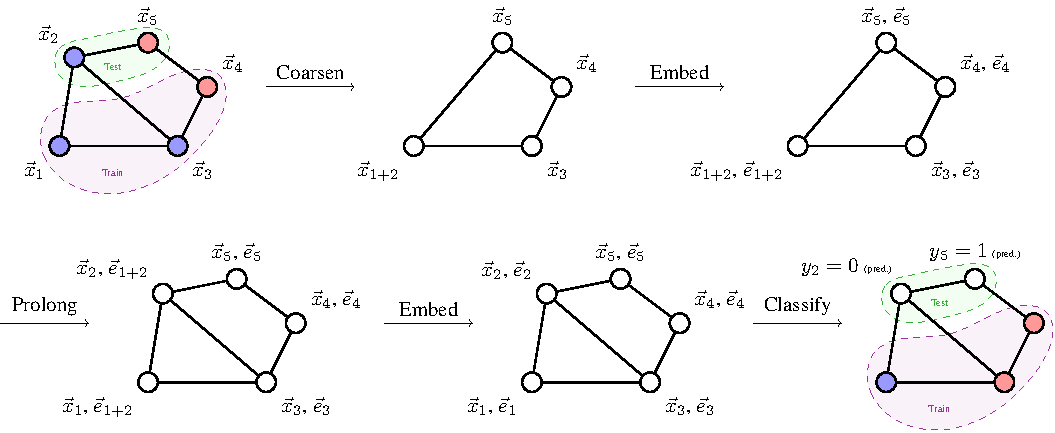
\includegraphics[width=0.8\textwidth]{images/harp-overview/harp-overview.pdf}
  \caption{An overview of the HARP processing pipeline with one level of coarsening}
  \label{fig:harp-overview}
\end{figure*}

\section{HARP extension for flexible performance-complexity balancing}\label{sec:our-method}

Graph representation learning methods such as node2vec typically have a large number of parameters -- on the widely used OGBN-ArXiv dataset (see \cite{hu_open_2021}), the state-of-the-art node2vec model has over 21 million parameters. At the same time, recent works in the domain of graph learning have started to focus more heavily on simpler methods as a competitive alternative to heavy-weight ones (see \cite{frasca_sign_2020,huang_combining_2020}). As the authors of \cite{chen_harp_2018} observed, HARP improves the performance of models when fewer labelled data are available. The proposed lower complexity models based on HARP could also improve performance in a setting where only low fidelity data are available for large parts of the graph. Coarser models could be trained on them, with a subsequent training of finer models using only a limited sample of high fidelity data.

In this work, we extend the general HARP framework to study the preformance-complexity characteristics of graph data. To this end, we propose alternatives to both the coarsening as well as the prolongation step of HARP. First, in Section~\ref{sec:adaptive-prolongation}, we replace the simple prolongation approach by an adaptive prolongation algorithm. Second, in Section~\ref{sec:coarsening-algorithms}, we study two alternative ways of coarsening the graph.

\subsection{Granularity of the HARP algorithm}

In standard HARP, once the coarsened graphs are obtained, the way to train the graph embedding is fairly straightforward. Starting with the coarsest graph, an embedding model such as node2vec is trained. Following that, a step to a graph that is one level finer is made. The embedding learned on the immediately preceding coarser graph is \name{prolonged} to the embedding of the following finer graph, in which the representations of merged nodes are copied and reused.
 Then, with this prolonged embedding as the starting state, the embedding algorithm continues training and this process is repeated until reaching the original graph.

While this style of prolongation is fine when HARP is used only as a means of pre-training, this approach is far too crude when studying the relationship between graph complexity and the quality of graph embedding and subsequent downstream applications. For example, the widely-used Cora dataset \cite{yang_revisiting_2016} has in its original form 2708 nodes, while the graph resulting from one application of the HARP coarsening schema has only about 1100 nodes (exact numbers may differ run-by-run). Such a relatively high reduction ratio effectively prevents any sufficient understanding of the relationship between graph reduction and changes in the quality of its embedding.

In order to offer a more fine-grained observation of the graph complexity and its effect on the downstream task, we present the adaptive prolongation approach. This algorithm works with the pre-coarsened graphs produced for example by HARP, however, the embedding is learned in a different manner.

\subsection{The adaptive prolongation approach}\label{sec:adaptive-prolongation}

\begin{figure}
  \centering
  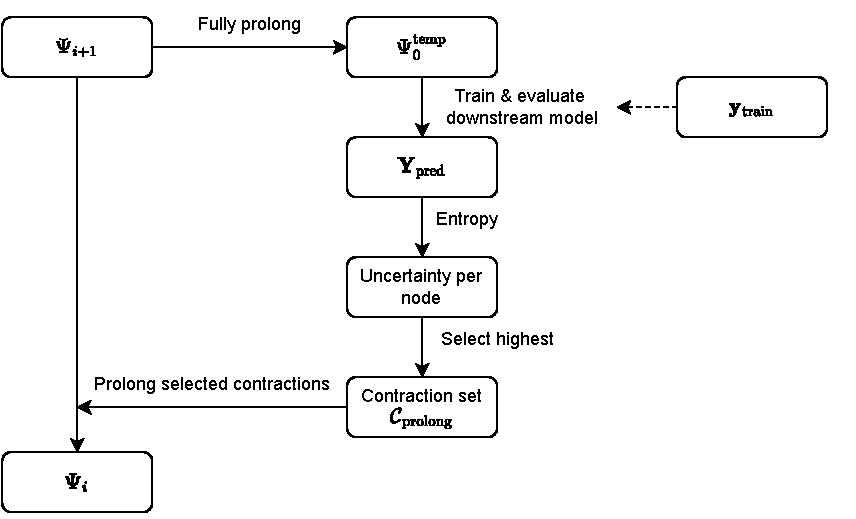
\includegraphics[width=\textwidth]{images/adaptive-prolongation/adaptive-prolongation.pdf}
    \caption{A schematic explanation of the adaptive prolongation algorithm for obtaining the embedding \( \Psi_{i} \) from \( \Psi_{i + 1} \).}
  \label{fig:adaptive-prolongation}
\end{figure}

The adaptive prolongation approach aims to replace the fixed steps defined by the used coarsening algorithm (such as HARP) by a variable number of smaller \enquote{micro-steps}, each of a predefined size that can be chosen independently from the underlying coarsening and its step size. Moreover, the prolongation procedure is driven by the interplay of the downstream task with the local properties of the underlying graph. This enables the method to produce embeddings with different level of granularity in different parts of the graph, e.g. an embedding that is coarse inside clusters of similar nodes and at the same time fine at the border between such clusters.

Let us denote \( \Psi_K, \dots, \Psi_0 \) the embedding sequence produced by the adaptive prolongation approach. To achieve the desired finer control over granularity the sequence \( \Psi_K, \dots, \Psi_0 \) needs to be decoupled from the graph sequence \( G_L, \dots, G_0 \), which in particular implies that the value of \( K \) is independent of \( L \). This is in contrast to the standard HARP prolongation, where the sequence of embeddings \( \Phi_{G_L}, \dots, \Phi_{G_0} \) is directly tied to the previously obtained graphs.

Similarly to standard HARP prolongation, the algorithm starts with the coarsest graph \( G_L \), trains a graph model to compute its embedding \( \Psi_K \) and gradually refines it until reaching the embedding \( \Psi_0 \) of \( G_0 \), or, alternatively, until a stopping criterion is met, as outlined in Section~\ref{sec:performance-complexity}. Instead of directly setting the value of \( K \), a fixed number of nodes \( n_p \) is prolonged in each step. These prolongation steps are interlaid with continued training of the graph model, as in standard HARP.  A description of a single prolongation step from \( \Psi_{i + 1} \) to \( \Psi_i \) follows, is schematically outlined in Figure~\ref{fig:adaptive-prolongation} and available as pseudocode in the supplementary material.

The procedure keeps track of all the edge contractions that were made in the dataset augmentation part of the algorithm and gradually reverses them. To this end, apart from the embedding \( \Psi_i \), the set of all contractions yet to be reversed as of step \( i \) is kept as \( \mathcal{C}_L^{(i)}, \dots, \mathcal{C}_0^{(i)} \), with the initial values \( \mathcal{C}_j^{(K)} \) corresponding to the underlying coarsening \( \varphi_j \) as defined in Section~\ref{sec:harp}.

In each prolongation step, the embedding \( \Psi_{i + 1} \) is prolonged to \( \Psi_i \) by selecting a set of \( n_p \) contractions \( \mathcal{C}_\mathrm{prolong} \) from the original coarsening procedure and undoing them by copying and reusing the embedding of the node resulting from the contraction to both of the nodes that were contracted. To obtain this set of contractions, nodes of \( G_0 \) are first ordered in such a way that corresponds to the usefulness of prolonging them. Subsequently, the set \( \mathcal{C}_\mathrm{prolong} \) is selected from \( \mathcal{C}_L^{(i + 1)}, \dots, \mathcal{C}_0^{(i + 1)} \) by selecting contractions affecting nodes in the aforementioned order, until \( n_p \) contractions are selected. If multiple contractions affecting the same node are available in the sequence \( \mathcal{C}_L^{(i + 1)}, \dots, \mathcal{C}_0^{(i + 1)} \), one is selected from \( \mathcal{C}_j^{(i + 1)} \) corresponding to the coarsest-level coarsening, that is, from \( \mathcal{C}_j^{(i + 1)} \) with the highest possible \( j \). The sequence \( \mathcal{C}_L^{(i)}, \dots, \mathcal{C}_0^{(i)} \) is produced from \( \mathcal{C}_L^{(i + 1)}, \dots, \mathcal{C}_0^{(i + 1)} \) by removing all of the edges contained in \( \mathcal{C}_\mathrm{prolong} \) (each edge from \( \mathcal{C}_\mathrm{prolong} \) will be contained in exactly one of \( \mathcal{C}_L^{(i + 1)}, \dots, \mathcal{C}_0^{(i + 1)} \)).

To obtain an ordering of nodes of \( G_0 \) based on the usefulness of their prolongation, the embedding \( \Psi_{i + 1} \) is fully prolonged to a temporary embedding of the full graph, \( \Psi_0^\mathrm{temp} \). A downstream model is then trained using this temporary embedding to obtain \( \mathmat{Y}_\mathrm{pred} \), the predicted posterior distribution of classes for each node in \( G_0 \) (e.g. the output of the softmax layer of an MLP). The entropy of this distribution is measured, representing the amount of uncertainty in the classifier for each given node. The nodes are ordered based on the entropy from highest to lowest. This reflects the principle that it is most useful to prolong those nodes where the downstream classifier is the least certain. For downstream tasks other than node classification, the ordering would need to be defined in a different manner, however the approach of prolonging the nodes about which the downstream model is the most uncertain can be extended to other tasks.

\subsection{More general approaches to coarsening}\label{sec:coarsening-algorithms}

While the adaptive prolongation approach substantially generalizes the original method into a powerful tool for studying and leveraging graph structure and its properties under a coarsening, it still relies on the pre-computed coarsenings to guide the prolongation process. In this section, we first present a brief overview of the coarsening algorithm as proposed by \cite{chen_harp_2018}, followed by two alternative proposals for coarsening construction based on graph diffusion.

\subsubsection{HARP coarsening}\label{sec:harp-coarsening}

The authors of \cite{chen_harp_2018} introduce two particular coarsening methods that together realize the function \( \varphi_i \) from Section~\ref{sec:harp} -- \name{edge collapsing} and \name{star collapsing}. Edge collapsing is a very simple method -- out of all the edges \( E \left( G \right) \), a maximal subset \( E' \) is selected randomly such that no two edges from \( E' \) are incident on the same node. Then, each edge in \( E' \) is contracted. Such an algorithm on its own is not sufficient to coarsen star-like structures with a high-degreen \textit{hub} node. To coarsen such structures effectively, the star collapsing algorithm pairwise merges the neighbours of such hub nodes, taking them in the order of decreasing node degree and never merging one node twice.

These two approaches are combined in the original HARP method, with each coarsening step being a star collapsing step followed by an edge collapsing step. Of a particular note is the fact that such a coarsening scheme cannot be constructed as a subset of edges of the graph. The star collapsing algorithm merges nodes that are adjacent to a common hub node, however, these nodes need not be connected by an edge. However, in our previously published work, we experimentally verified that the star collapsing algorithm can be replaced by a similar algorithm that repeatedly merges nodes adjacent on a hub node with the hub node itself.

\subsubsection{Graph diffusion coarsening}\label{sec:gdc-coarsening}

Our definition of a graph coarsening requires choosing some edges from the original graph. Intuitively, one way of constructing a graph coarsening would be to merge nodes which are similar and therefore no significant amount of information is lost due to such a coarsening. Following both of these premises, we propose a coarsening based on Graph Diffusion Convolution (GDC) \cite{gasteiger_diffusion_2019} algorithm. GDC is a general graph transformation which, in an overview, constructs for a given graph a new edge set, represented by a so-called sparsified generalized graph diffusion matrix \( \hat{\mathmat{S}} \), which would, in the original setting of the method, be used as a replacement for the adjacency matrix of the graph. To apply this algorithm as a way of coarsening the graph, the edge set obtained by GDC is intersected with the edges of the original graph and the resulting edges contracted in the graph, i.e.,
\[ \mathcal{C} = E \left( G_{\hat{\mathmat{S}}} \right) \cap E \left( G \right), \]
using the construction of a graph coarsening as a subset of its edges, as presented in Section~\ref{sec:harp}.

In principle, the authors of GDC define the generalized graph diffusion matrix
\begin{equation}\label{eq:gdc-matrix}
    \mathmat{S} = \sum_{k = 1}^\infty \theta_k \mathmat{T}^k
\end{equation}
such that the power series converges. The parameters \( \theta_k \) together with the generalized transition matrix \( \mathmat{T} \) define the exact way in which the diffusion is achieved. Among the choices for \( \mathmat{T} \) is the random walk transition matrix \( \mathmat{T}_ \mathrm{rw} = \mathmat{A} \mathmat{D}^{-1} \) and the symmetric transition matrix \( \mathmat{T}_\mathrm{sym} = \mathmat{D}^{-\frac{1}{2}} \mathmat{A} \mathmat{D}^{-\frac{1}{2}} \) where \( \mathmat{D} \) is the diagonal matrix of node degrees. Two special cases of this general schema using the random walk transition matrix are the Personalized PageRank algorithm (PPR) \cite{page_pagerank_1999} and the heat kernel \cite{kondor_diffusion_2002}.

Graph sparsification needs to be used in order to preserve reasonable computational requirements throughout the diffusion. In GDC, two such methods are considered -- thresholding the matrix values and selecting top-\( k \) entries for each column of the matrix. In any case, the matrix is normalized after sparsification, thus finally producing \( \hat{\mathmat{S}} \).

\section{Experimental evaluation}\label{sec:experimental-evaluation}

\subsection{Experiment setup}

\subsubsection{Datasets}

The proposed methods were experimentally verified on several datasets. The datasets Cora and CiteSeer \cite{yang_revisiting_2016} were used with the \enquote{full} train-test split as in \cite{chen_fastgcn_2018}. In addition, 2 variants of the Twitch dataset \cite{rozemberczki_multi-scale_2021} with the hignest node count (DE and EN) were used. Five medium sized datasets were also used, the PubMed dataset \cite{yang_revisiting_2016}, the DBLP dataset \cite{bojchevski_deep_2018}, the IMDB dataset \cite{xinyu_magnn:_2020} and both variants of the Coauthor dataset \cite{shchur_pitfalls_2019}. Finally, one large dataset was used, the OGB ArXiv dataset \cite{weihua_open_2021}.

\subsubsection{Methodology of experiments}

The hyper-parameters for both the node2vec model used for the embedding training and the multi-layer perceptron used for downstream classification were initially set to values used in prior art (see \cite{hu_open_2021,fey_fast_2019}) and then manually fine-tuned for each dataset.

The achitecture of the algorithm was identical accross the dataset, with the only difference being in the values of the hyper-parameters, as listed in Table~\ref{tab:hyperparameter-values}. For the Cora dataset, the node2vec model generated an embedding in \( \mathfield{R}^{128} \) from \( 4 \) random walks of length \( 20 \) for each node with a context window of size \( 5 \). The optimizer ADAM \cite{kingma_adam:_2017} was used with a learning rate of \( 0.01 \) and batches of \( 128 \) samples. The model was trained for \( 5 \) epochs and in each step of the adaptive prolongation, \( 100 \) nodes were prolonged, until reaching the original graph (the value of \( n_p \) was calculated so that the total number of training epochs would match baseline model training). The MLP classifier using the embeddings featured \( 3 \) linear layers of \( 128 \) neurons with batch normalization after each layer. Each layer was normalized using dropout \cite{srivastava_dropout_2014} with the rate of \( 0.5 \). Finally, a linear layer was used for the class prediction. For the classifier, ADAM with a learning rate of \( 0.01 \) was used for \( 30 \) epochs of training with the cross-entropy loss function. Dataset features weren't used for the classifier training as the aim of this work is to compare the embeddings. The experiment was run \( 10 \) times end-to-end and results averaged. The experiments were implemented using PyTorch \cite{paszke_pytorch_2019} and PyTorch Geometric \cite{fey_fast_2019}.

\begin{table*}
  \caption{Hyper-parameter values used for different datasets}
  \label{tab:hyperparameter-values}
  \centering
  \begin{tabular}{lrrrrrrrr}
    \toprule
    \textbf{Hyper-parameter} & \textbf{Cora} & \textbf{CiteSeer} & \textbf{PubMed} & \textbf{DBLP} & \textbf{Twitch} & \textbf{IMDB} & \textbf{ArXiv} & \textbf{Coauthor} \\
    \midrule
    Embedding dimension      & 128           & 32                & 64              & 32            & 128             & 128           & 128            & 128               \\
    \# of random walks       & 4             & 5                 & 3               & 2             & 10              & 40            & 10             & 40                \\
    Random walk length       & 20            & 20                & 40              & 20            & 80              & 100           & 80             & 10                \\
    Context window size      & 5             & 5                 & 20              & 5             & 3               & 5             & 20             & 5                 \\
    Node2vec learning rate   & 0.01          & 0.01              & 0.01            & 0.01          & 0.025           & 0.01          & 0.01           & 0.01              \\
    Node2vec batch size      & 128           & 128               & 128             & 128           & 128             & 256           & 128            & 256               \\
    Node2vec epochs          & 5             & 7                 & 1               & 1             & 5               & 1             & 1              & 1                 \\
    %\# of prolonged nodes    & 100           & 150               & 1000            & 800           & 200             & 1400          & 8000           & 1250              \\
    \# of MLP layers         & 3             & 3                 & 1               & 3             & 2               & 2             & 3              & 2                 \\
    MLP hidden layer width   & 128           & 256               & 128             & 256           & 64              & 64            & 256            & 16                \\
    Dropout rate             & 0.5           & 0.5               & 0.5             & 0.5           & 0.5             & 0.5           & 0.5            & 0.5               \\
    MLP learning rate        & 0.01          & 0.01              & 0.01            & 0.01          & 0.01            & 0.01          & 0.01           & 0.01              \\
    MLP epochs               & 30            & 80                & 300             & 300           & 500             & 100           & 300            & 100               \\
    \bottomrule
  \end{tabular}
\end{table*}

\subsection{Evaluation of the adaptive approach}\label{sec:adaptive-experiments}

In order to study the effect of the adaptive prolongation, the adaptive prolongation method was used to assess the performance of downstream transductive classification at different coarsening levels. A node2vec model as described in the previous section was trained with adaptive prolongation based on coarsenings pre-computed by the HARP coarsening algorithm as described in \ref{sec:harp-coarsening}. For each prolongation step, the intermediary embedding was afterwards fully prolonged to obtain an embedding of the original graph \( G \) (as that is the only graph for which ground-truth labels are available). A classifier was then trained with this embedding as input. This setup allows us to compare classification accuracy at each step of the adaptive prolongation. Figure~\ref{fig:adaptive-coarsening} shows the results of this experiment, compared with a baseline node2vec model (that is, without any coarsening or prolongation) that was trained for the same number of epochs as the total epochs of the adaptive model over all prolongation steps.

\begin{figure*}
  \centering
  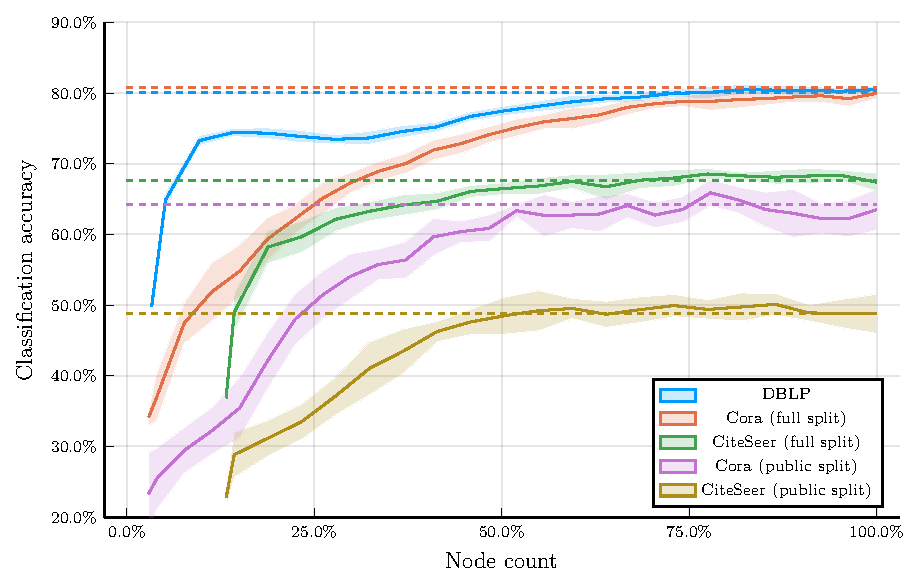
\includegraphics[width = \linewidth]{images/adaptive-coarsening/adaptive-coarsening.pdf}
  \caption{Downstream classifier accuracies at different steps of adaptive prolongation using the basic HARP coarsening algorithm. Dashed line shows the baseline node2vec model accuracy. The node count is taken relative to the total node count in each dataset. The results are averaged over multiple runs, with the solid line representing the mean and the shaded area denoting one standard deviation.}
  \label{fig:adaptive-coarsening}
\end{figure*}

The behaviour of the model somewhat differs between the used datasets. For the Cora, CiteSeer, DBLP, PubMed, ArXiv and Coauthor datasets, the model starts from a very low performance, which quickly rises as the model trains for several prolongation steps. The model trained on CiteSeer attains performance comparable to the reference model when approximately half of all nodes are available to it. On the other hand, with e. g. Coauthor-CS, the model slowly approaches the reference model for the whole duration of training, only reaching comparable performance at a point where nearly the whole graph is available to it. Models trained on the two medium-sized datasets, DBLP and PubMed, exhibit a different behaviour in that they briefly reach a local maximum followed by a slight decrease in performance until finally approaching the performance of the reference model in a manner similar to the models trained on Cora and CiteSeer. The ArXiv dataset exhibits a similar behaviour to a lesser extent. This behaviour is further discussed in the next section. The Twitch and IMDB datasets are substantially different, with very high initial performance and only small performance gains with increasing number of nodes available, with different variants of it exhibiting this effect to a different magnitude.

To further study the model properties from a statistical point of view, the results were evaluated at \( k \)-th deciles of the node count of the full graph, for all possible values of \( k \). At each decile, the performance of the model was compared to the baseline node2vec model using the Wilcoxon signed-rank test with the Holm-Bonferroni correction for multiple hypothesis testing with the hypothesis that the models are equivalent. The hypotheses were rejected by the test at the 5\% level of significance for \( k \in \left\{ 1, 2, 3, 4, 5 \right\} \), suggesting that the adaptive prolongation approach is valid and practically useful in situations where at least half of the nodes is available.

Following recent best-practice recommendations regarding verifying the statistical validity of results \cite{benavoli_time_2017}, the results were also studied from the point of view of Bayesian estimation. Similarly to the frequentist approach, the performance of the model was compared to that of the baseline model at \( k \)-th deciles of the node count, for all possible values of \( k \). The comparison was done using the Bayesian Wilcoxon signed-rank test \cite{benavoli_bayesian_2014} for 3 different widths of the region of practical equivalence (ROPE), 1\%, 5\% and 10\%. The probabilities that the two models are practically equivalent are listed in Table~\ref{tab:bayesian-adaptive}. Of a particular note is the fact that at 60\% complexity, the models have over a 99\% probability of being within 10 percentage points of performance -- showing that the proposed method may offer a significant complexity reduction in exchange for a relatively minor decrease in performance.

\begin{table}
  \caption{The probabilities that the adaptive approach will be practically equivalent to node2vec when compared on different fractions of the full graph and with different widths of the region of practical equivalence.}
  \label{tab:bayesian-adaptive}
  \centering
  \begin{tabular}{lrrr}
    \toprule
    \textbf{Nodes} & \textbf{1\% ROPE} & \textbf{5\% ROPE} & \textbf{10\% ROPE} \\
    \midrule
    \textbf{10\%}  & 0\%               & 0.3\%             & 2.5\%              \\
    \textbf{20\%}  & 0\%               & 0.8\%             & 14.1\%             \\
    \textbf{30\%}  & 0\%               & 1.7\%             & 35.3\%             \\
    \textbf{40\%}  & 0\%               & 5.3\%             & 72.0\%             \\
    \textbf{50\%}  & 0.1\%             & 35.3\%            & 85.7\%             \\
    \textbf{60\%}  & 0.6\%             & 62.2\%            & 99.7\%             \\
    \textbf{70\%}  & 32.0\%            & 84.7\%            & 100.0\%            \\
    \textbf{80\%}  & 30.0\%            & 99.9\%            & 100.0\%            \\
    \textbf{90\%}  & 48.9\%            & 100.0\%           & 100.0\%            \\
    \textbf{100\%} & 87.7\%            & 100.0\%           & 100.0\%            \\
    \bottomrule
  \end{tabular}
\end{table}

\subsection{The relationship of the results and the properties of the graph}

When the models for DBLP and PubMed are studied more closely, both reach a local maximum at around 14\% of the graph, followed by a slight decline and gradual approach to the baseline. This suggests a global structure in the data, which the model learns at the point of the local maxima. To investigate this hypothesis and try to explain the behaviour of the model in general, several graph metrics were applied to the graphs generated during the adaptive prolongation algorithm run. All of the metrics were applied to the graph \( G_i \) at each step in the prolongation process.

The metrics used were edge homophily \cite{zhu_beyond_2020}, node homophily \cite{pei_geom-gcn_2020}, class homophily \cite{lim_large_2021}, adjusted homophily \cite{platonov_characterizing_2022}, balanced accuracy \cite{platonov_characterizing_2022}, adjusted accuracy \cite{platonov_characterizing_2022}, label informativeness \cite{platonov_characterizing_2022}, and global assortativity \cite{newman_mixing_2003}.

The values of these metrics were compared to the classification accuracy and a strong correlation was found for the majority of them, with correlation coefficient of \( -0.66 \) for global assortativity and between \( 0.94 \) and \( 0.96 \) for all the other metrics, averaged across the datasets. This suggests the explanation of the graphs being heterophilic when very coarse (as could be expected), then reaching a point where the global structure of the graph is in place and is then only refined in a local sense. Such a behaviour may introduce nodes which have a different label than their neighbourhoods (a kind of noise in the data), which is a possible explanation for the local optima in performance.

\subsection{Comparison of coarsening approaches}

For GDC coarsening, only the top-\( k \) sparsification method produces reliable results as thresholding leads to instability in the coarsening process, either collapsing the whole graph almost immediately, or not collapsing it at all. As for the other parameters, we followed \cite{gasteiger_diffusion_2019}. Both of the diffusion methods propsed in \cite{gasteiger_diffusion_2019} were implemented with the recommended parameter values, that is the heat kernel was used with the diffusion time \( t = 5 \) and the Personalized PageRank algorithm with the teleport probability \( \alpha = 0.15 \) and the recommended normalization. To be able to compute graph diffusion for larger graphs, approximate diffusion algorithms were used. For PPR, a version of the Andersen algorithm \cite{andersen_local_2006} with \( \epsilon = 10^{-2} \) was used and for heat kernel diffusion, a version of the Kloster-Gleich algorithm \cite{kloster_heat_2014} with \( \epsilon = 10^{-5} \) was used. Both of these algorithms were modified to produce edge weights as part of their output.

The behaviour of the models was compared in average over all datasets, comparing their node classification accuracy relative to that of the baseline node2vec model. A statistical analysis of the results follows and the full plot of accuracies of all models on all datasets is available in the supplementary material, however, in general, both the GDC as well as the PPR coarsening outperform the model with  HARP coarsening. On average, GDC has \( 8\% \) higher accuracy than the HARP model at \( k \in \left\{ 1, 2 \right\} \), \( 7\% \) higher accuracy at \( k = 3 \) and \( 3\% \) higher accuracy at \( k = 4 \). For higher values of \( k \), the differences are negligible. For PPR, the accuracies are on average \( 13\%, 17\%, 7\%, 7\% \) higher for \( k \in \left\{ 1, 2, 3, 4 \right\} \), respectively.

Statistical tests similar to the ones described in Section~\ref{sec:adaptive-experiments} were carried out to compare the different models. The Friedmann two-way analysis of ranks with the Holm-Bonferroni correction was used to test the hypothesis that all of the methods are equivalent at \( k \)-th deciles for all possible values of \( k \). This hypothesis was rejected for \( k \in \left\{ 1, 2, 3, 4, 5, 6 \right\} \) with Holm-corrected familywise p-values \( 1.84 \times 10^{-7}, 1.84 \times 10^{-7}, 1.51 \times 10^{-10}, 1.51 \times 10^{-10}, 8.13 \times 10^{-5}, 9.66 \times 10^{-3} \), respectively. For these deciles, a post-hoc pairwise Wilcoxon test was performed between the HARP, PPR and heat kernel methods. At the 5\% significance level, the test did not reject the hypothesis that any two coarsening algorithms are equivalent for any \( k \).

The coarsening approaches were also compared using Bayesian estimation, using the Bayesian Wilcoxon signed-rank test in a pairwise fashion for all possible values of \( k \) with a 5\% region of practically equivalence. When comparing HARP to the heat kernel, the probability of HARP having higher accuracy was less than \( 3\% \) for all values of \( k \). On the other hand, the probability of the heat kernel having higher accuracy was \( 34\%, 25\%, 13\%, 1\% \) for \( k \in \left\{ 1, 2, 3, 4 \right\} \) respectively. For other values of \( k \), the probability that the models are practically equivalent was over \( 96\% \). When comparing HARP and PPR, for \( k \in \left\{ 1, 2, 3, 4, 5 \right\} \), the probability of HARP having higher accuracy was \( 9\%, 8\%, 10\%, 10\%, 8\% \), respectively. The probability of the PPR having higher accuracy was \( 67\%, 47\%, 33\%, 35\%, 13\% \) for \( k \in \left\{ 1, 2, 3, 4, 5 \right\} \), respectively, leaving the remainder as probability of the two methods being practically equivalent. For all other values of \( k \), the methods have over 99\% probability of being practically equivalent. When comparing the heat kernel and PPR, both methods have over \( 95\% \) probability of being practically equivalent for \( k > 5 \). For lower values of \( k \), neither method has over \( 35\% \) probability of having higher accuracy then the other, with both methods having higher probability for some values of \( k \). The results show that all the methods are practically equivalent when the graph is only slightly coarsened and at higher levels of coarsening, GDC and PPR dominate HARP coarsening, with the particular choice between them being dataset-dependent.

\section{Conclusion}

In this work, a general graph coarsening schema modelled on the basis of the HARP algorithm was proposed. A novel approach to prolonging graphs in the HARP setting was presented, yielding an adaptive algorithm that selectively prolongs the graph in a way that maximizes performance of the considered downstream task under limited graph size. Additionally, 2 alternatives to HARP coarsening based on graph diffusion were presented. Together, these two improvements substantially increase the versatility of HARP, turning it from a method for pre-training into a framework for graph reduction. Such a framework enables the study of properties of particular graphs, making it possible to reveal global structures. The framework may be used for lowering computational demands while preserving downstream task performance as well.

All of the proposed methods were experimentally verified. While the behaviour differs between the graphs studied, in general, our experiments reveal that at about 50\% reduction in node count, the accuracy was still reasonably close to the accuracy on a full graph for most datasets. Additionally, the coarsenings based on graph diffusion were shown to outperform the original coarsening, again with the exact difference depending on the particular dataset and coarsening level.

In future work, a simpler, direct way of tackling the performance-complexity trade-off problem for graphs may be studied as an alternative to the approach proposed in this work. Our preliminary exploration of this direction studies the setting of direct adaptive coarsening, instead of a fixed coarsening followed by adaptive prolongation.


\subsubsection{Acknowledgements}

The research reported in this paper has been supported by the German Research Foundation (DFG) funded project 467401796.

\bibliographystyle{splncs04}
\bibliography{zotero}

\end{document}
